\documentclass[10pt]{article}
\usepackage{graphicx}
\usepackage{float}
\usepackage{listings}
\usepackage{xcolor}
\usepackage{caption}
\usepackage{algorithm}
\usepackage{algpseudocode}

\definecolor{codegreen}{rgb}{0,0.6,0}
\definecolor{codegray}{rgb}{0.5,0.5,0.5}
\definecolor{codepurple}{rgb}{0.58,0,0.82}
\definecolor{backcolour}{rgb}{0.95,0.95,0.92}

\lstdefinestyle{mystyle}{
    backgroundcolor=\color{backcolour},   
    commentstyle=\color{codegreen},
    keywordstyle=\color{magenta},
    numberstyle=\tiny\color{codegray},
    stringstyle=\color{codepurple},
    basicstyle=\ttfamily\footnotesize,
    breakatwhitespace=false,         
    breaklines=true,                 
    captionpos=b,                    
    keepspaces=true,                 
    numbers=left,                    
    numbersep=5pt,                  
    showspaces=false,                
    showstringspaces=false,
    showtabs=false,                  
    tabsize=2,
    frame=single
}

\lstset{style=mystyle}

\title{Generación de Patrones Sintéticos: Chessboard y Spiral}
\author{Brandon Marquez Salazar}
\date{Universidad de Guanajuato \\ \today}

\begin{document}

\maketitle

\section{Introducción}

Este trabajo presenta la implementación de dos patrones sintéticos: un tablero de ajedrez y un patrón espiral.

\section{Métodos}

\subsection{Generación de Patrones Sintéticos}

Se implementaron dos patrones: chessboard y spiral. El primero funcionó correctamente, el segundo presentó problemas en su implementación.

\subsubsection{Patrón Chessboard}

El patrón chessboard se genera como una matriz $M$ de $n \times m$ píxeles. Cada cuadro tiene dimensiones $w \times h$. El algoritmo sigue un patrón alternante basado en la paridad de las filas.

\begin{algorithm}
\caption{Generación de Chessboard}
\begin{algorithmic}[1]
\Procedure{Chessboard}{$n, m, w, h$}
\State $M \gets 255$ \Comment{Inicializar blanco}
\For{$i = 0$ \textbf{to} $n-1$}
    \State $j_{start} \gets (i \bmod 2) \cdot w$
    \For{$j = j_{start}$ \textbf{to} $m-1$ \textbf{step} $2w$}
        \For{$x = 0$ \textbf{to} $w-1$}
            \For{$y = 0$ \textbf{to} $h-1$}
                \State $M[i \cdot h + y, j + x] \gets 0$
            \EndFor
        \EndFor
    \EndFor
\EndFor
\State \Return $M$
\EndProcedure
\end{algorithmic}
\end{algorithm}

La implementación en C++ utiliza un enfoque similar con bucles anidados:

\begin{lstlisting}[language=C++, caption=Implementación Chessboard]
void chessboard(cv::Mat& image, const lovdog::dummystruct& dummy){
  size_t x,y, i, j, a;
  image.create(dummy.chess_height * dummy.chess_rows,
               dummy.chess_width * dummy.chess_cols, CV_8UC1);
  
  i=0; while(i<(size_t)image.rows){
    j=0; while(j<(size_t)image.cols) 
      image.at<uchar>(i,j++)=255; 
    ++i; 
  }
  
  i=0; while(i<dummy.chess_rows){
    j=(i&1)*dummy.chess_width;
    while((int)j<image.cols){
      a=i*dummy.chess_height;
      x=0; while(x < dummy.chess_width){
        y=0; while(y < dummy.chess_height){
          image.at<uchar>(a+(y++),j+x) = 0;
        }
        ++x;
      } 
      j+=2*dummy.chess_width;
    } 
    ++i;
  }
}
\end{lstlisting}

\subsubsection{Patrón Spiral: Planificación del Algoritmo}

Para el patrón spiral, se planeó un algoritmo que siguiera un rastro similar a un barbechado, evitando cruzar las restricciones de los márgenes. La idea central era usar un índice circular sobre un vector con los cuatro movimientos posibles para lograr un avance fluido.

La matriz $M \in \mathbb{R}^{n \times m}$ no es necesariamente cuadrada. Sea $g$ el grosor de la línea que formará la espiral y también el espacio entre sus paredes.

Los márgenes se calculan como:
\begin{itemize}
    \item Margen superior: $m_{sp} = \lfloor m \bmod g \rfloor$
    \item Margen inferior: $m_{in} = m \bmod g - m_{sp}$
    \item Margen izquierdo: $m_{iz} = \lfloor n \bmod g \rfloor$
    \item Margen derecho: $m_{dr} = n \bmod g - m_{iz}$
\end{itemize}

El punto de inicio es $P_i = (m_{iz}, m_{sp})$. El cambio de dirección siempre es a la derecha, usando un índice circular sobre el vector de movimientos $\vec{d} = \{(1,0), (0,1), (-1,0), (0,-1)\}$.

Los rangos para cada caso se definen como:

\begin{algorithm}
\caption{Planificación del Algoritmo Spiral}
\begin{algorithmic}[1]
\Procedure{Spiral}{$n, m, g$}
\State $M \gets 255$ \Comment{Fondo blanco}
\State Calcular $m_{sp}, m_{in}, m_{iz}, m_{dr}$
\State $P \gets (m_{iz}, m_{sp})$ \Comment{Punto inicial}
\State $\vec{d} \gets \{(1,0), (0,1), (-1,0), (0,-1)\}$
\State $idx \gets 0$ \Comment{Índice direccional}
\State $a,b,c,d \gets 0$ \Comment{Contadores de ajuste progresivo}
\While{espacio disponible}
    \If{dirección horizontal}
        \State $x \in [a + m_{iz}, m_{dr} - b]$ \Comment{Rango horizontal}
        \State $y \in [c + m_{sp}, c + m_{sp} + g]$ \Comment{Grosor vertical}
        \State Dibujar línea horizontal
        \State $c \gets c + g$ \Comment{Ajustar para siguiente segmento}
    \Else
        \State $x \in [a + m_{iz}, a + m_{iz} + g]$ \Comment{Grosor horizontal}
        \State $y \in [c + m_{sp}, m_{in} - d]$ \Comment{Rango vertical}
        \State Dibujar línea vertical
        \State $a \gets a + g$ \Comment{Ajustar para siguiente segmento}
    \EndIf
    \State $idx \gets (idx + 1) \bmod 4$ \Comment{Cambio cíclico de dirección}
    \State Actualizar $b,d$ según corresponda
\EndWhile
\State \Return $M$
\EndProcedure
\end{algorithmic}
\end{algorithm}

La idea del barbechado consiste en que cada vez que se completa un segmento horizontal o vertical, los contadores $a,b,c,d$ se incrementan en $g$, haciendo que el área disponible para el siguiente segmento se reduzca. Esto crea el efecto de espiral que se va cerrando progresivamente.

El punto de inflexión para cambiar la dirección ocurre cuando el algoritmo encuentra el límite de sus posibles movimientos, detectado por las condiciones de los rangos. La transición entre direcciones debe ser suave, manteniendo la continuidad del patrón.

\section{Resultados}

\subsection{Patrón Chessboard}

El algoritmo de chessboard generó el patrón esperado. La figura muestra el resultado con parámetros $w=40$, $h=20$, $8\times8$ cuadros.

\begin{figure}[H]
    \centering
    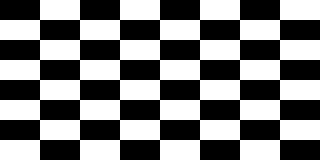
\includegraphics[width=0.7\textwidth]{chessboard.png}
    \caption{Patrón chessboard generado por el algoritmo.}
    \label{fig:chessboard}
\end{figure}

El patrón muestra alternancia correcta entre cuadros blancos y negros. Los bordes son nítidos y las dimensiones se mantienen consistentes en toda la imagen.

\subsection{Patrón Spiral}

La implementación del patrón spiral no funcionó correctamente. Aunque la planificación del algoritmo era sólida en teoría, la implementación práctica presentó problemas con la sincronización de los contadores $a,b,c,d$ y la detección precisa de los puntos de inflexión.

El algoritmo generaba segmentos desconectados o patrones que no correspondían a una espiral cerrada. La transición entre direcciones no era suave y en ocasiones se producían solapamientos o huecos en el patrón.

\section{Conclusiones}

El patrón chessboard se implementó correctamente usando un enfoque basado en paridad de filas. Para el patrón spiral, la planificación teórica con el sistema de barbechado y ajuste progresivo de contadores era adecuada, pero la implementación requirió un manejo más cuidadoso de las transiciones entre segmentos y la sincronización de los límites.

\end{document}
